\documentclass[12pt,a4paper]{report}

\usepackage[utf8x]{inputenc}
\usepackage{amsmath}
\usepackage{amsfonts}
\usepackage{amssymb}
\usepackage{graphicx}
\usepackage{enumitem}
\usepackage{pgf}
\usepackage{tikz}
\usepackage{calrsfs}
\usetikzlibrary{arrows,automata,calc}

\begin{document}

\begin{titlepage}
	\centering
	{\scshape\LARGE Universidad Autónoma de México \par}
	\vspace{1cm}
	{\scshape\Large Computación Distribuida\par}
	\vspace{1.5cm}
	{\huge\bfseries Tarea I\par}
	\vspace{.5cm}
	{\Large\itshape Edgar Quiroz Castañeda \par}
    \vspace{.5cm}
	{\Large\itshape Jerónimo Almeida Rodríguez \par}
	\vfill
	 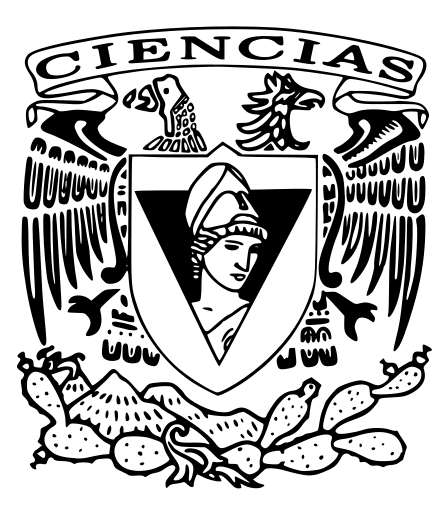
\includegraphics[width=0.5\textwidth]{escudo_f-ciencias.png}
	\vfill

% Bottom of the page
	{\large Jueves 23 de Agosto del 2018 \par}
\end{titlepage}

\pagebreak
\setlength{\voffset}{-0.75in}
\setlength{\headsep}{5pt}

\newcommand{\ed}[2]{(#1) edge (#2)}
\newcommand{\eee}[4]{\path [->,draw,thin] ($ (#1) !.5! (#2)$) -- ($ (#3) !.5! (#4) $);}


\begin{enumerate}
		%Ejercicio 1
		\item {
		Dada la siguiente gráfica $\mathcal{O}$, propón una tarea distribuida
		$T=\langle \mathcal{I}, \mathcal{O}, \Delta \rangle$ con salida $\mathcal{O}$.
		Describe el significado de todas las configuraciones iniciales en $T$
		utilizando alguna situación de la vida real, como los ejemplos con Alice y
		Bob vistos en clase y también describe a $\Delta$.\\
		\begin{center}
		  \begin{tikzpicture}[-,>=stealth',auto, node distance = 2.8cm, 
				shorten > = 1pt, semithick, state/.style = {circle, fill=#1,
				draw=black!, inner sep=1mm, text=black}, state/.default = white]

			 \tikzstyle{every state}=[fill=white,draw=black!,text=black]

		  	 \node (AO0) [state]                      {$(A,0)$};%E
		  	 \node (BO0) [state=gray, right of=AO0]   {$(B,0)$};%F
		     \node (BO3) [state=gray, below of=AO0]   {$(B,\frac{1}{3})$};%G
		  	 \node (AO2) [state, below of=BO3]        {$(A,\frac{2}{3})$};%H
		  	 \node (BO1) [state=gray, below of=AO2]   {$(B,1)$};%I
		   	 \node (AO3) [state, below of=BO0]        {$(A,\frac{1}{3})$};%J
		  	 \node (BO2) [state=gray, below of=AO3]   {$(B,\frac{2}{3})$};%K
		  	 \node (AO1) [state, below of=BO2]        {$(A,1)$};%L

		  	 \path  \ed{AO0}{BO0}
					\ed{AO0}{BO3}
					\ed{BO3}{AO2}
					\ed{AO2}{BO1}
					\ed{BO0}{AO3}
					\ed{AO3}{BO2}
					\ed{BO2}{AO1}
					(AO1) edge node {$\mathcal{O}$} (BO1);

		  \end{tikzpicture}
		\end{center}
		
		La tarea que proponemos es la siguiente: \\
		\begin{tikzpicture}[-,>=stealth',auto,
		node distance = 2.8cm,
		    shorten > = 1pt, semithick,
		 state/.style = {circle, fill=#1, draw=black!,
		                 inner sep=1mm, text=black},
		 state/.default = white]

		  \tikzstyle{every state}=[fill=white,draw=black!,text=black]

		  \node (AI0) [state]                      {$(A,0)$};%A
		  \node (BI0) [state=gray, right of=AI0]   {$(B,0)$};%B
		  \node (AI1) [state, below of=BI0]        {$(A,1)$};%C
		  \node (BI1) [state=gray, below of=AI0]   {$(B,1)$};%D
		  \node (AO0) [state, above right of=BI0]  {$(A,0)$};%E
		  \node (BO0) [state=gray, right of=AO0]   {$(B,0)$};%F
		  \node (BO3) [state=gray, below of=AO0]   {$(B,\frac{1}{3})$};%G
		  \node (AO2) [state, below of=BO3]        {$(A,\frac{2}{3})$};%H
		  \node (BO1) [state=gray, below of=AO2]   {$(B,1)$};%I
		  \node (AO3) [state, below of=BO0]        {$(A,\frac{1}{3})$};%J
		  \node (BO2) [state=gray, below of=AO3]   {$(B,\frac{2}{3})$};%K
		  \node (AO1) [state, below of=BO2]        {$(A,1)$};%L

		  \path \ed{AI0}{BI0}
			    \ed{BI0}{AI1}
			    \ed{AI0}{BI1}
			    (AI1) edge node {$\mathcal{I}$} (BI1)
				\ed{AO0}{BO0}
				\ed{AO0}{BO3}
				\ed{BO3}{AO2}
				\ed{AO2}{BO1}
				\ed{BO0}{AO3}
				\ed{AO3}{BO2}
				\ed{BO2}{AO1}
				(AO1) edge node {$\mathcal{O}$} (BO1);

		  \eee{AI1}{BI1}{BO1}{AO1}
		  \eee{AI0}{BI0}{AO0}{BO0}
		  \eee{AI0}{BI1}{AO0}{BO3}
		  \eee{AI0}{BI1}{BO3}{AO2}
		  \eee{AI0}{BI1}{AO2}{BO1}
		  \eee{AI0}{BI1}{AO0}{BO3}
		  \eee{AI1}{BI0}{AO3}{BO0}
		  \eee{AI1}{BI0}{BO2}{AO3}
		  \eee{AI1}{BI0}{AO1}{BO2}

		\end{tikzpicture}
	}
	\item {
	Dado el problema del inciso anterior, propón un álgoritmo en el modelo de
	comunicación siguiente y demuestra que es correcto.\\\\
		\begin{equation*}
			\mathcal{M} = \{A \leftrightarrow B, A \rightarrow B, A \leftarrow B \}
		\end{equation*}
	}
\end{enumerate}
\end{document}
